% ICSE 2027 Industry Challenge -- Solution paper for Challenge #7:
% "Log-Guided Root-Cause Code Localization from Production Issues"
% Track rules: 5-10 pages incl. figures/tables/appendices + max 2 pages refs,
% IEEEtran 10pt conference (no compsoc), double-anonymous.
% Submission: https://icse2027-industry-challenge.hotcrp.com  (Nov 13, 2026 AoE)
\documentclass[10pt,conference]{IEEEtran}

\usepackage[T1]{fontenc}
\usepackage[utf8]{inputenc}
% IEEEtran sets subsection titles in italic, and \sys{} is small caps, so
% a heading like \subsection{\sys{}} asks Times for small-caps-italic --
% a shape it does not have. LaTeX already falls back to small caps; this
% declares that substitution so it stops warning on every build.
\DeclareFontShape{T1}{ptm}{m}{scit}{<->ssub*ptm/m/sc}{}
\DeclareFontShape{T1}{ptm}{b}{scit}{<->ssub*ptm/b/sc}{}
\usepackage{graphicx}
\usepackage{booktabs}
\usepackage{amsmath}
\usepackage{xspace}
\usepackage{xcolor}
\usepackage[hidelinks]{hyperref}
\usepackage[capitalise]{cleveref}
% the best value in a column of the all-systems table, when it is ours
\definecolor{win}{RGB}{0,110,0}
\newcommand{\win}[1]{\textcolor{win}{\textbf{#1}}}
% Table bodies are generated by scripts/paper_tables.py into tables/*.tex.
% LaTeX's \input cannot sit inside a tabular row (its file-exists check
% leaves a token that breaks \bottomrule); the primitive can.
\makeatletter
\newcommand{\tablebody}[1]{\@@input tables/#1.tex }
\makeatother

% --- macros: single source for every headline number -------------------------
% Every value below is on the 27-project benchmark (seed 42, one run).
% Sources: paper/benchmark-numbers.md (datasheet), c7_coverage.py on the
% merged wf rows (agent), the same paired with the loop-ablation main run,
% data/results/agentic-baselines.json (the 1,000-instance sample), and
% paper_numbers.py (pooled retrieval, function and dense numbers).
\newcommand{\sys}{\textsc{Remember}\xspace} % working name, can change
\newcommand{\retr}{the retrieval layer\xspace}  % lexical+memory pipeline; a tool inside the agent
\newcommand{\nInstances}{38{,}001\xspace}   % mined
\newcommand{\nScored}{37{,}900\xspace}      % after the test-only-gold exclusion
\newcommand{\nProjects}{27\xspace}
\newcommand{\nHardPct}{49\%\xspace}         % benchmark-wide
\newcommand{\nMemoryPool}{172{,}331\xspace} % sum of data/benchmark/<p>-memory.jsonl
% The agent is evaluated on the WHOLE evaluation split, not a sample.
\newcommand{\nEval}{26{,}544\xspace}
\newcommand{\nEvalHard}{12{,}799\xspace}
\newcommand{\accOne}{68.6\%\xspace}
\newcommand{\accFive}{85.9\%\xspace}
\newcommand{\mrr}{0.761\xspace}
\newcommand{\hardOne}{52.8\%\xspace}
\newcommand{\hardFive}{73.6\%\xspace}
\newcommand{\modOne}{90.2\%\xspace}         % the agent's own module answer
\newcommand{\nRegion}{24{,}850\xspace}      % eval instances with a derivable gold function
\newcommand{\regOne}{53.8\%\xspace}
\newcommand{\regFive}{69.9\%\xspace}
% the retrieval layer on the same 26,544 instances
\newcommand{\retrOne}{41.2\%\xspace}
\newcommand{\retrFive}{70.3\%\xspace}
\newcommand{\retrHardFive}{48.7\%\xspace}
% the unconstrained-loop ablation (same model, same evidence pass) on the same instances
\newcommand{\loopOne}{67.9\%\xspace}
\newcommand{\loopFive}{86.8\%\xspace}
\newcommand{\loopRegOne}{39.8\%\xspace}
\newcommand{\loopRegFive}{50.7\%\xspace}
% cost per issue
\newcommand{\calls}{15.7\xspace}
\newcommand{\tokens}{106k\xspace}
% the 1,000-instance sample for the agent baselines
\newcommand{\nSample}{1{,}000\xspace}
\newcommand{\nSampleHard}{483\xspace}
% memory firewall: share of candidate votes removed by the future-reports
% rule, pooled over the 27 projects (memory_vote_stats in <p>-summary.json)
\newcommand{\firewallPct}{63\%\xspace}
% module level (tables/modules.tex, paper_tables.py)
\newcommand{\moduleRetr}{76.5\%\xspace}    % tables/modules.tex, module-metrics.json pooled
\newcommand{\moduleFreq}{49.3\%\xspace}    % module-baselines.json, most_frequent_live pooled

\begin{document}

\title{Log-Guided Root-Cause Code Localization from Production Issues:\\
A Staged Agent Evaluated on 26{,}544 Real Incidents}

\author{\IEEEauthorblockN{Anonymous Author(s)}}

\maketitle

\begin{abstract}
When a production issue is reported, engineers receive a description
and logs, but no failing test and no way to reproduce the fault. The
logs show where the failure was detected, not where it was caused: in
\nHardPct{} of the real reports we study, no file touched by the
eventual fix is named anywhere in the text.
We mined a benchmark for this setting from two public issue datasets
and \nProjects{} git histories: \nInstances{} incidents from Apache
projects, MongoDB, MariaDB, Qt and Sakai, each pairing a report and its
logs with the code at a revision where the defect is still present and
the files the fix later changed, plus a per-project pool of
\nMemoryPool{} resolved issues that serves as an \emph{incident memory}
behind a temporal firewall.
We present \sys{}, a localization agent that reads code with a
general-purpose 27B open-weights model inside a fixed, staged
procedure: code gathers the evidence, including the files that similar
past incidents were fixed in, and the model decides only which files to
open, what role each file plays in the failure, and the order of the
files. Every step is bounded, every decision is recorded, and the run
cannot end without a module, ranked code regions and a causal chain.
On the whole \nEval{}-instance evaluation split \sys{} ranks a file the
fix changed first for \accOne{} of incidents and in the top five for
\accFive{}, names the affected module for \modOne{}, and names a
function the fix changed first for \regOne{}; on the half of the
reports that name no faulty file it reaches \hardOne{} and \hardFive{}.
An ablation with the same model and tools in an unconstrained agent
loop finds files equally well but names the faulty function fourteen
points less often and cites no log event in its explanations. On a
\nSample-instance sample
it leads reimplementations of two published localization agents by 7
and 20 points of Acc@1 (4 and 16 on the instances the ports answered),
the same model used alone by 14, and the same model used as a re-ranker
by 6, all differences significant, and the
model cannot recall these public fixes from the issue key alone. We
report the cost of every system and the results that go against us.
The benchmark, both systems, every run transcript and a script that
traces each number to its result file are released.
\end{abstract}

\begin{IEEEkeywords}
log analysis, fault localization, root cause analysis, incident management
\end{IEEEkeywords}

\section{Introduction}
\label{sec:intro}

When a production issue is reported, an engineer typically receives two
things: a natural-language description of what went wrong, and logs. There
is no failing test, no debugger session, and often no way to reproduce the
problem. From this evidence alone, the engineer must find the code that
caused it. The challenge this paper answers calls for techniques that
perform this step automatically: given an issue report, logs, and a source
code snapshot, produce the affected module, a ranked list of suspicious
code regions, and the evidence that connects them.

The core difficulty is that logs show where a failure was \emph{detected},
not where it was \emph{caused}. A real example from our benchmark makes
this concrete. Kafka issue KAFKA-6624 reports that a disk is wrongly
marked offline, and its stack trace points at
\texttt{FileChannelImpl.force} and \texttt{FileRecords.flush}, the code
that hit a closed file channel. The actual fix landed in
\texttt{LogManager.scala}, which allowed a log to be deleted while it was
still being flushed. Every file the trace names is innocent. Any method
that works by matching the report against the code it mentions, which is
what an engineer grepping the codebase does, starts from the wrong files.
In our benchmark, \nHardPct{} of real reports name none of the files the
fix later touched.

Existing techniques approach this from two sides, and both stop short.
Classical fault localization ranks suspicious code using failing tests or
coverage, execution evidence that does not exist at report
time~\cite{just2014defects4j}. Recent agent-based variants retrieve over
the codebase itself~\cite{rafi2024multiagent}, treating every issue as if
it were the project's first. Log-based root cause analysis in cloud
operations~\cite{wang2024rcagent} identifies the faulty service or
component, but stops above the level of code regions.

One source of evidence is missing from both: the project's own resolved
history. Software failures recur. When an issue arrives, some past issue
has often failed in a similar way, and its fix commit records exactly
which files were at fault that time. We call this \emph{incident
memory}. Past incidents whose reports resemble the new one vote for the
files their fixes touched. A memory used carelessly would cheat, because
the history of a project contains fixes that did not exist when the
report was filed, so every use of it here sits behind a temporal
firewall that admits only incidents resolved before that moment.

Studying any of this required a benchmark that was not available: issue
reports with logs, the code as it was when the issue was open, and
ground-truth faulty files. We mined one from two public datasets and
project git histories. It contains \nInstances{} real incidents from four
projects of four organizations (Apache Kafka, MariaDB, MongoDB, Qt),
where the ground truth of each instance is the set of source files its
fix commit modified, and the snapshot is the parent of that commit. The
benchmark is stratified by exactly the difficulty the challenge names:
whether the report names any faulty file.

We then use the benchmark to compare four families of method on the same
instances, under one protocol and one firewall: classic
information-retrieval bug localization, lexical log-to-code retrieval
fused with incident memory, a general-purpose open 27B model prompted
with the report and the file tree, and that model used to re-rank
retrieved candidates. Accuracy in the top five rises across the families
from $0.180$ to $0.839$. The more useful result is that no family
dominates. Retrieval alone and the model alone solve different
instances: retrieval is the only one of the two to succeed on 6.1\% of
instances, the model alone on 21.1\%, and the union of their top-five
lists reaches $0.892$ where each alone reaches $0.681$ and $0.832$.

That gap between what the parts find separately and what either finds
alone is the opening this paper takes. We present \sys{}, an agent that
keeps the retrieval and the incident memory as tools and adds tools that
read code, resolve a symbol from a stack trace to the file that defines
it, and consult past incidents behind the same firewall. \sys{} runs on
the same 27B model used in the study, so what it adds is the
architecture, not a larger model. Kafka issue KAFKA-7693 shows the
pattern. The report is a crash on a negative sequence number, and
retrieval returns nothing useful. \sys{} resolves the symbol in the
trace, reads the code that produces that number, and ranks
\texttt{TransactionManager.java} first, the file whose arithmetic
creates the negative value. On 105 of the 375 hard instances it ranks the
faulty file first where retrieval does not place it in the top five at
all.

This paper makes four contributions.
\begin{itemize}
\item \textbf{A benchmark} of \nInstances{} issue--log--code--fix
  instances across four organizations, with a per-filter datasheet and a
  per-project incident-memory pool, released for reuse
  (\cref{sec:benchmark}).
\item \textbf{A comparative study} of four families of localization
  method on those instances, under one protocol and one temporal
  firewall (\cref{sec:results}). It reports what each family achieves,
  where each fails, and that they fail on different instances. It also
  measures what the firewall is worth: the classic similar-report
  signal, evaluated without report-time admissibility, overstates Acc@5
  by 9\% to 43\% relative (\cref{sec:results:leakage}).
\item \textbf{\sys{}}, an agent that turns the retrieval, the incident
  memory, and the code itself into tools (\cref{sec:agent}). It reaches
  Acc@5 $0.903$ and Acc@1 $0.723$, improving on every family in the
  study and on the best combination of them, with the widest margins on
  the reports that name no faulty file. Its cost is reported next to its
  accuracy.
\item \textbf{Three validity checks} that a reviewer of an
  LLM-based result should expect, each of which could have invalidated
  the result and did not (\cref{sec:results:validity}). The model cannot
  recall these public fixes from the issue key alone. Shuffling the
  order of the retrieved candidates changes no outcome. Every baseline
  is rescored on the exact instances the agent ran, because the
  evaluation sample is easier than the full split.
\end{itemize}

The lexical parts of the system are deterministic, and the agent's tools
are pure functions of the snapshot, so a recorded run replays to
identical tool results. Every reported number traces to a result file
through a released script.

\section{A Benchmark from Issues, Logs, and Fix Commits}
\label{sec:benchmark}

The challenge asks for evaluation on a benchmark that contains issue
descriptions, logs, source code, and ground-truth faulty code regions.
Existing resources supply some of these but not the combination we need.
Fault localization benchmarks such as Defects4J~\cite{just2014defects4j}
supply failing tests, which is exactly the execution evidence that is
missing when an issue is first reported. Bench4BL pairs reports with
code and gold files at scale but does not select for reports that carry
logs~\cite{lee2018bench4bl}, and benchmarks built from pull
requests~\cite{aleithan2024swebenchplus} inherit solution text in the
issue thread. Pathidea assembled the closest resource, a log-bearing
set of Java issues~\cite{chen2022pathidea}.

What we add is a set selected for log-bearing reports, spanning four
languages rather than one, stratified by whether the report names any
faulty file, and shipped with a per-project pool of past incidents and
their fix commits so that history-based methods can be evaluated under a
stated temporal firewall. This section describes how each instance is
constructed and what quality controls we applied.

\subsection{Data sources}
\label{sec:benchmark:sources}

We join two public datasets. The first is World of Logs v2 (WoL), a
dataset of software logs extracted from online documents~\cite{wang2026wol}.
For every public Jira issue it records whether the issue text contains
log messages, and an uncertainty score for that extraction. The second is
The Public Jira Dataset v7 (PJD)~\cite{montgomery2022jira}, which provides
the complete metadata of 2.7 million issues from 16 public Jira trackers,
including creation time, resolution time, resolution status, and typed
links between issues. WoL is itself built on PJD, so the two join exactly
on the issue key. Both datasets are licensed CC-BY-4.0, which allows us to
redistribute the benchmark with attribution.

From the 16 trackers we selected four projects: Apache Kafka (Java and
Scala), MariaDB server (C and C++), MongoDB server (C++), and Qt
(C++, the \texttt{qtbase} module). The four projects come from four
different organizations and two tracker platforms, and they differ
strongly in how their users report bugs, as \cref{sec:benchmark:strata}
shows.

\subsection{From an issue to its ground truth}
\label{sec:benchmark:linkage}

An issue enters the benchmark if it satisfies four conditions. First, its
text contains logs according to WoL, with extraction uncertainty at most
0.05, the threshold the WoL authors recommend. Second, it is a bug: its
issue type is \emph{Bug} and its resolution is \emph{Fixed} or
\emph{Done}. Third, it can be linked to the commit that fixed it. For
Kafka, MariaDB, and MongoDB, developers put the issue key in the commit
subject (for example, ``KAFKA-10089 The stale ssl engine factory is not
closed after reconfigure''). Qt developers instead record the key in a
\texttt{Fixes:} trailer in the commit message. We scan the default branch
of each project's repository and keep issues linked to one to three
commits. Issues linked to more commits are long-running efforts rather
than single faults, and we drop them. We also drop revert commits and
merge commits, whose diffs do not describe a single fix. Fourth, the fix
must change source code: at least one modified file must be a non-test
source file of the project's main languages.

For every surviving issue, the \emph{ground truth} (gold) is the set of
non-test source files that the fix commit modified. The \emph{code
snapshot} is the repository at the parent of the fix commit. This is the
code as it existed while the bug was still present, so the fix itself is
never visible to a localization method. The \emph{query} is the issue
summary and description, truncated at 20{,}000 characters. This matches
the challenge input: a natural-language report with the logs the reporter
pasted into it.

\begin{table}[t]
\caption{Benchmark datasheet. ``Eligible'' counts log-bearing fixed bugs
(conditions 1 and 2); ``linked'' additionally requires a clean fix-commit
link (condition 3); ``final'' requires modified non-test source files
(condition 4). ``Hard'' instances do not name any gold file in their
text. The memory pool (\cref{sec:benchmark:memory}) does not require
logs, so it is larger than the benchmark itself.}
\label{tab:datasheet}
\centering
\begin{tabular}{lrrrr}
\toprule
 & Kafka & MariaDB & MongoDB & Qt \\
\midrule
Eligible issues        & 1{,}172 & 3{,}004 & 6{,}407 & 7{,}412 \\
Linked (1--3 commits)  & 827     & 2{,}010 & 5{,}093 & 713 \\
Final instances        & 680     & 1{,}683 & 3{,}618 & 456 \\
\midrule
Hard stratum           & 28\%    & 44\%    & 60\%    & 68\% \\
With stack trace       & 47\%    & 57\%    & 10\%    & 24\% \\
Single fix commit      & 91\%    & 83\%    & 80\%    & 96\% \\
Gold files (median)    & 1       & 1       & 2       & 1 \\
\midrule
Memory pool            & 4{,}033 & 6{,}014 & 19{,}820 & 2{,}315 \\
\bottomrule
\end{tabular}
\end{table}

\Cref{tab:datasheet} reports the yield of every condition. The final
benchmark holds 6{,}437 instances, of which 6{,}314 are scored; the
123 we leave unscored, and why, are described in
\cref{sec:setup:populations}. The largest loss differs by project
and is informative in itself. Qt loses most instances at the linkage
step, because its tracker covers about forty repositories and we mine
only \texttt{qtbase}. MongoDB loses most at the source-file step, because
many of its fixes change only test or build files.

\subsection{Easy and hard instances}
\label{sec:benchmark:strata}

The challenge notes that error logs often show where a failure was
detected rather than where it originated. Our benchmark makes this
measurable. We call an instance \emph{easy} if the issue text mentions
the name of at least one gold file, for example in a pasted stack trace.
We call it \emph{hard} otherwise: the report describes the failure, but
no gold file is named anywhere in it. Across the benchmark, 53\% of
instances are hard. The fraction varies strongly by project
(\cref{tab:datasheet}). Kafka reports often contain a Java stack trace
that names the faulty class, so only 28\% are hard. Qt reports describe
misbehaving user interfaces and rarely contain a trace, so 68\% are hard.
Every result in this paper is reported on both strata. We also record
whether each instance contains a stack trace at all, which supports the
same analysis from the input side.

The definition is file-based, and that choice is not language-neutral:
a Java frame names the file (class and file coincide), while a C++
frame names a function. To bound this artifact we computed a second
definition that also counts a mention of a gold file's basename stem or
of any function defined in a gold file. The hard fraction then falls to
14\% (Kafka), 33\% (MariaDB), 38\% (MongoDB), and 38\% (Qt): part of
the Java-to-C++ gap is indeed the naming convention, and the three C++
projects converge to a band of 33\% to 38\% while Kafka stays well
below it. We
keep the file-based definition for stratification because a file name
is what grep turns into a candidate file directly, but both labels ship
with the benchmark.

\subsection{The incident memory pool}
\label{sec:benchmark:memory}

Our approach uses the project's resolved history as a signal
(\cref{sec:approach}). This history does not need logs: any fixed issue
whose fix commit we can identify tells us which files a past problem
ended in. We therefore build a separate \emph{memory pool} per project
from all of PJD, using conditions 2 to 4 but not condition 1. Each pool
entry carries the issue's summary and description, its creation and
resolution timestamps, its fix commits, and the gold files of those
commits. The pools are between three and six times larger than the benchmarks
(\cref{tab:datasheet}). PJD's typed issue links also give us duplicate
clusters: groups of issues marked as duplicates of one another. We use
the timestamps and the clusters to keep the memory honest during
evaluation (\cref{sec:approach:firewall}).

\subsection{Limitations of mined ground truth}
\label{sec:benchmark:limits}

Mined gold is not perfect, and we state its known weaknesses. A commit
subject can mention an issue it does not fix, although our filters remove
the most common cases (reverts, merges, and multi-commit efforts). A fix
can touch files beyond the faulty one, for example during a small
refactoring; the median fix modifies one to two source files, which
bounds this effect. Finally, the file a fix modifies is the place the
developers chose to repair, which is occasionally not the place the
defect originated. We accept these imperfections because they are the
same imperfections real resolved histories have. A method that works on
this benchmark works on what projects actually record.

\section{Approach: Log-to-Code Retrieval Plus Incident Memory}
\label{sec:approach}

Our approach, \sys{}, follows one observation: software failures recur.
When a new issue arrives, some past issue in the same project has often
failed in a similar way, and its fix commit names the code that was at
fault. \sys{} therefore combines two kinds of evidence. The first is
\emph{log-to-code retrieval}: matching the report's text and logs against
the snapshot's files. The second is \emph{incident memory}: retrieving
similar resolved incidents and letting their fix commits vote for files.
This section describes both, the firewall that keeps the memory honest,
and the fusion that produces the final ranking.

\subsection{Overview}
\label{sec:approach:overview}

The input matches the challenge: an issue report with its logs, and the
code snapshot. The output is a ranked list of the snapshot's source
files, the affected module derived from that list, and, for every ranked
file, the evidence that put it there. Four signals each produce a ranked
list over the snapshot's non-test source files. A weighted fusion merges
the four lists into one. All components run on CPU, use no training, and
are deterministic: the same input always yields the same ranking.

\subsection{Log-to-code signals}
\label{sec:approach:signals}

\textbf{Trace mentions (S1).} The most direct evidence is a file named in
the report itself. S1 finds explicit mentions: file names with an
extension (\texttt{KafkaChannel.java}, \texttt{row0mysql.cc:123}) and
class names inside stack-trace frames (\texttt{at
org.apache.kafka...}). Mentioned files are ranked by where they first
appear in the text, since reporters tend to paste the decisive trace
early. If the text names no file explicitly, S1 falls back to counting
occurrences of bare file-name stems. S1 is deliberately simple because it
doubles as a baseline: it is the automated form of an engineer grepping
the report.

\textbf{Path retrieval (S2).} Path names carry meaning: a report about a
stale SSL factory shares words with
\texttt{security/ssl/SslFactory.java}. S2 scores every file path against
the report with BM25, a standard lexical ranking function, after
splitting identifiers on case and underscores.

\textbf{Content retrieval (S3).} The strongest textual evidence sits
inside the files: identifiers, string literals, and the logging
statements that produced the reported log lines. Scoring every file's
content in every snapshot would be slow and, worse, would tempt a global
index that leaks information across time. S3 therefore scores a
per-instance candidate pool: the files found by S1, the top 200 files
from S2, and the files proposed by memory (below). Term statistics are
computed inside this pool only, so nothing from any other snapshot or any
later version influences the score.

\subsection{The incident memory signal}
\label{sec:approach:memory}

\textbf{Memory retrieval and voting (S4).} S4 searches the project's
memory pool (\cref{sec:benchmark:memory}) for past incidents whose
summary and description read like the current report, again with BM25
over an inverted index. The twenty most similar admissible incidents then
vote: an incident at similarity rank $r$ adds $1/r$ to every gold file of
its own fix commit, provided that file still exists in the current
snapshot. The intuition is the on-call engineer's: ``this looks like the
broker bug from last spring, and that one ended in
\texttt{KafkaChannel}.'' Unlike S1 to S3, S4 can point at a file that no
log line and no trace ever names, which is exactly what the hard stratum
requires.

\subsection{The memory firewall}
\label{sec:approach:firewall}

A memory signal evaluated on historical data can cheat in ways that are
invisible if they are not controlled. We exclude a past incident from
voting on a query when any of the following holds, and we count every
exclusion:

\begin{enumerate}
\item it is the query issue itself;
\item it belongs to the query's duplicate cluster, so it describes the
  same incident under another key;
\item it shares a fix commit with the query, which happens when one
  commit closes several issues;
\item it was resolved after the query was created. The memory an
  engineer could actually search at report time contains only incidents
  resolved before the report existed.
\end{enumerate}

Rule 4 is strict and it costs real signal: in our runs it blocks roughly
two thirds of candidate votes. We accept the cost because the remaining
signal is one a deployed system would truly have had.

\subsection{Fusion, modules, and evidence}
\label{sec:approach:fusion}

\textbf{Weighted fusion.} The four lists are merged by reciprocal rank
fusion: file $f$ receives $\sum_i w_i / (60 + \mathrm{rank}_i(f))$, where
$\mathrm{rank}_i(f)$ is $f$'s position in signal $i$'s list. The weights
$w_i$ are the only tuned parameters in \sys{}.

\textbf{Conditioning on an observable regime.} The right weights depend
on the report. When the text names files explicitly, S1 is nearly always
right and should dominate. When it names none, S1 is noise and memory
matters more. The easy/hard strata of \cref{sec:benchmark:strata} cannot
be used for this decision, because they are defined through the gold
answer. We instead condition on a property that is visible at inference
time: whether S1 found at least one explicit file mention. Weights are
tuned separately for the two regimes, by grid search over
$\{0, 0.5, 1, 2\}$ per signal, on a development split only
(\cref{sec:setup:protocol}). The ablation without memory is tuned the
same way, so the comparison in \cref{sec:results} is fair to both sides.

\textbf{Module and evidence outputs.} The affected module is read off the
file ranking: files collapse to their leading path components (one to
three, fixed per project since two of the four keep all code under
\texttt{src/}), and a module's rank is the rank of its first file. For
the explanation output, every ranked file carries its provenance: which
signals ranked it, the matching log lines or mentions for S1 to S3, and
for S4 the past incidents that voted for it with their issue keys. An
engineer can follow these links directly to the prior fix.

\section{\sys{}: a staged investigation}
\label{sec:agent}

\begin{figure*}[t]
\centering
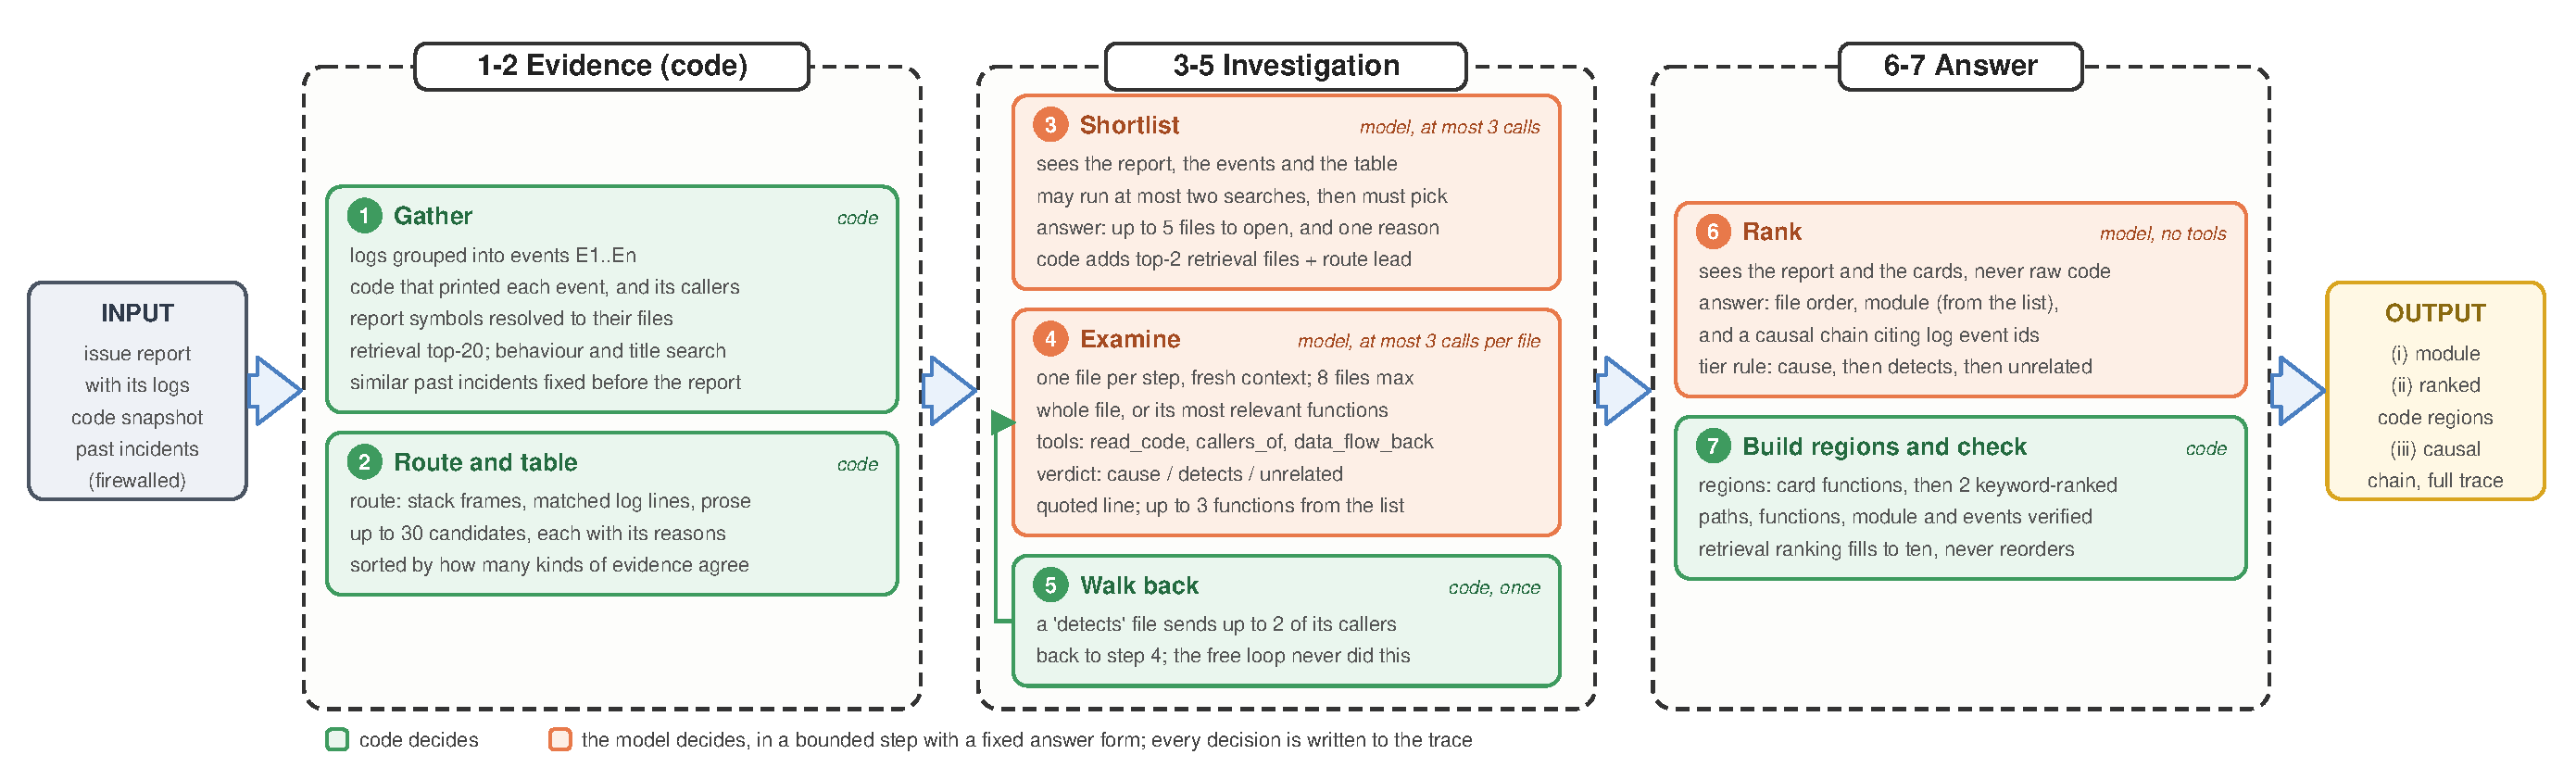
\includegraphics[width=0.98\textwidth]{figures/workflow.pdf}
\caption{\sys{}. Code gathers the evidence and builds a candidate table
(1, 2). The model then makes three kinds of decision, each in a bounded
step with a fixed answer form: which files to open (3), what role one
file plays (4, one file per step, the code on screen), and the order of
the files (6, from the verdict cards only). Code walks back from files
that only detect the failure (5) and checks the answer (7). Green steps
are code; orange steps are the model.}
\label{fig:workflow}
\end{figure*}

\sys{} runs on one general-purpose 27B open-weights model, self-hosted,
at temperature zero with a fixed seed. Its inputs are the issue report
with its logs, the code snapshot, and the project's incident memory
behind the firewall of \cref{sec:approach:firewall}. Its outputs are
the affected module, a ranked list of code regions (file and
function), and a chain of steps from the reported
symptom to the named cause, each step citing a log event from the
report where one applies.

\subsection{Design principles}
\label{sec:agent:principles}

Localization agents are usually built as a loop: one model, a set of
tools, a turn budget, and the model deciding at every turn what to do
next and when to stop. \sys{} is built on four principles that take
those decisions away from the model. The evidence is gathered by code
before the model is called, so no turn is spent searching for what the
report already names. Every candidate file is judged on its own, in a
fresh context with its code on screen, so a file's rank depends on what
its code does rather than on how often or how recently it was read.
The step from a file that only detects a failure to the files that
could have caused it is taken by code, not left to the model. And the
run ends when the procedure ends, with a submission the schema requires
to be complete. What this structure is worth is measured in
\cref{sec:results:structure} against an ablation that gives the same
model the same tools in an unconstrained loop.

\subsection{The staged workflow}
\label{sec:agent:stages}

\Cref{fig:workflow} shows the procedure. It is fixed; the model decides
only inside it, three times, and every decision is written to the
trace.

\textbf{1. Gather (code).} Code collects the evidence before the model
is called. The logs in the report are grouped into events and labelled
\texttt{E1}, \texttt{E2}, \ldots; for each event the code finds the
statement that printed it and that statement's callers; every symbol in
the report is resolved to the file that defines it; the retrieval layer
of \cref{sec:approach} supplies its top twenty files; the incident
memory is queried, behind the firewall, for similar past incidents and
the files their fixes touched; a behaviour search and a title search run
over file content.

\textbf{2. Route and table (code).} The report is routed by what it
contains: stack frames, else log lines that match a statement in the
code, else prose. Every file any channel named goes into one candidate
table of up to thirty rows, each with the reasons it is there
(``declares \texttt{SequenceNumber}'', ``fixed in past incident
KAFKA-5342'', ``prints log event E2''). The table is sorted by how many
kinds of evidence point at a file.

\textbf{3. Shortlist (model, at most three calls).} The model sees the
compressed report, the events and the table, may run at most two
searches if the table clearly misses the described behaviour, and must
answer with up to five paths to examine. Code keeps only paths that are
in the table or that the model's own searches returned, and always adds
the top two retrieval files and the route's lead file, whether or not
the model picked them.

\textbf{4. Examine (model, one file per step, at most three calls
each).} Each queued file is judged alone, in a fresh context that holds
only the report and that file: the whole file when it fits 24{,}000
characters, otherwise its most relevant functions whole, most relevant
first, until the budget is full, plus the list of every function the
file declares. The model may read another part of the same file, list a
symbol's callers, or ask where a value is set, and must answer with a
fixed-form verdict: the file's role (\emph{cause}: code here creates
the bad state; \emph{detects}: code here only reports or checks a bad
state made elsewhere; \emph{unrelated}), up to three function names
copied from the list, and the line the verdict rests on. A function name
the file does not contain is dropped, never repaired. At most eight
files are examined per run.

\textbf{5. Walk back (code, once).} For every file judged to
\emph{detect} the failure, code looks up the callers of the function the
verdict named and sends up to two caller files back to step 4.

\textbf{6. Rank (model, no tools).} The model sees the report and the
verdict cards, never raw code or tool output, and answers with the order
of the files, the affected module copied from the snapshot's module
list, and the causal chain, each step naming a log event id or none.
Code then applies one rule the prompt also states: files judged
\emph{cause} come before \emph{detects}, and those before
\emph{unrelated}, with the model's order kept inside each group.

\textbf{7. Build regions and check (code).} Regions are built per file
in rank order: the card's functions first (two for each of the first
three files, one after that), then two functions ranked by keyword
match against the report, marked as such. Every path must exist in the
snapshot, every function in its file, the module in the module list, and
every cited log event in the report; a citation that fails is removed.
If fewer than ten files were examined, the retrieval ranking fills the
remaining file slots without reordering what the agent produced.

The whole run spends \calls{} model calls on average: one to restate
the symptom in code vocabulary during gathering, up to three to
shortlist, up to three per examined file, and one or two to rank. The
model is never asked to remember what it read in an earlier step,
because every step receives what it needs in full, and it is never
asked to decide when to stop, because the procedure stops.

\subsection{Reproducing an agent}
\label{sec:agent:repro}

Every tool is a pure function of the snapshot, the memory pool and the
query, so a recorded run replays to identical tool results, and every
run is persisted in full: each prompt, each response, each decision and
its reason, the cards, and the final answer. What is not reproducible is
the model: under continuous batching the composition of a batch changes
the order of floating-point reductions, so two runs of one instance with
the same seed can return different text. We measured that variation
rather than assuming it away, and report it with the results
(\cref{sec:results:negatives}). No tool can reach the ground truth: the
gold files of the instance under investigation are not in the memory
pool, in any index, or on any path a tool will read.

\section{Evaluation Setup}
\label{sec:setup}

This section fixes the protocol: how the benchmark is split, what is
measured, which systems are compared, and how significance is decided.

\subsection{Time-based split}
\label{sec:setup:protocol}

Each project's instances are ordered by the time of their fix commit. The
earliest 30\% form the development split, and the later 70\% form the
evaluation split. All tuning, which in \sys{} means only the fusion
weights of \cref{sec:approach:fusion}, happens on the development split.
Every number reported in \cref{sec:results} comes from the evaluation
split. We chose a time split rather than a random one because it mirrors
deployment: a system is configured on the project's past and then meets
the project's future. A random split would let instances from the future
inform the configuration used on the past.

The time split has a side effect worth recording, because any system that
uses historical memory will meet it. The development split holds the
oldest issues, and the oldest issues have the least history behind them.
Tuned on that slice, the fusion weights undervalue memory relative to its
worth on later data. We report this as a property of the protocol and
keep the split anyway; the alternative, tuning on recent data and
evaluating on older data, would be the deployment scenario backwards.

\subsection{Metrics}
\label{sec:setup:metrics}

We report the challenge's metrics at the file level: Acc@K, the fraction
of instances with at least one gold file in the top $K$; Recall@K, the
average fraction of an instance's gold files found in the top $K$; and
MRR, the mean reciprocal rank of the first gold file. We use
$K \in \{1, 5, 10\}$ and treat Acc@5 as primary, since five files is a
realistic number for an engineer to open. At the module level we report
Acc@K and MRR for the module ranking defined in
\cref{sec:approach:fusion}; the function-level stage of
\cref{sec:results:functions} reuses the same metrics over function
candidates.

\subsection{Compared systems}
\label{sec:setup:systems}

Each signal from \cref{sec:approach} runs standalone as a baseline:
trace mentions (S1), path retrieval (S2), content retrieval (S3), and
memory alone (S4). S1 represents what an engineer gets by grepping the
report. On top of these we evaluate the fused system in two forms,
unweighted fusion and regime-conditioned weighted fusion, and each form
both with and without the memory signal. The without-memory variants are
tuned with the same grid and the same development split as the full
system, so the memory ablation compares two equally tuned systems rather
than a tuned system against a crippled one.

We additionally re-implement the classic IRBL baselines, since the
original tools are Java-only. \textbf{rVSM} scores every file of the full
snapshot with a length-favoring tf--idf cosine. \textbf{BugLocator}
combines rVSM with SimiScore, the 2012 similar-report
signal~\cite{zhou2012buglocator}: every past fixed report votes for its
fix's files with weight $\mathrm{sim}(q,b)/n_b$; the blend weight uses
the replication-standard $\alpha = 0.3$, with
$\alpha \in \{0.2, 0.3, 0.5\}$ tuned on the development split as a
variant. \textbf{BRTracer-style} adds the stack-trace boost of
BRTracer~\cite{wong2014brtracer} ($+1/r$ for the file at trace rank
$r \le 10$); we omit the original's file segmentation and state so. Unless noted otherwise, their SimiScore runs
under the SAME firewall as our memory signal, so the comparison is honest
on both sides; \cref{sec:results:leakage} measures what happens without
it.

\subsection{Statistical treatment}
\label{sec:setup:stats}

Every comparison in \cref{sec:results} is tested with a paired bootstrap
over instances: 2{,}000 resamples, identical resample indices for all
comparisons within a population, two-sided $p$-values from the bootstrap
distribution, and 95\% confidence intervals. The paper reports two test
families, each corrected with the Benjamini--Hochberg procedure over the
whole family: 64 tests for the main comparisons (four comparisons, two
metrics, two populations, four projects) and 96 tests for the baseline
and leakage experiment of \cref{sec:results:leakage} (six comparisons,
same grid). We call a result significant only when the corrected
$q < 0.05$. The pipeline itself is deterministic from end to end: fixed
seeds, greedy decisions, and no GPU training. Re-running every experiment
reproduces every table in this paper bit for bit, and the released
artifact contains a script that traces each reported number to the result
file it came from.

\section{Results}
\label{sec:results}

Every number in this section is from the \nProjects-project benchmark.
The agents and the retrieval layer are scored on the full \nEval-instance
evaluation split; the two reimplemented published agents, which cost
more to run, are scored on a stratified \nSample-instance sample of that
split (\cref{sec:setup:populations}). All systems in one table are
scored on identical instances. Intervals are 95\% paired bootstrap
intervals over instances; ``significant'' means the interval excludes
zero. Every agent number comes from one run with one seed; what that
costs in precision is measured in \cref{sec:results:negatives}.

\begin{table*}[t]
\caption{File, module and region localization on the full evaluation
split (\nEval{} instances, \nEvalHard{} of them hard, meaning the report
names no file the fix changed). The three systems share the same
evidence pass; the two agents also share the model. Region metrics are
on the \nRegion{} instances whose fix diff yields a gold function.
Cost is per issue: model calls / prompt tokens.}
\label{tab:headline}
\centering
\footnotesize
\setlength{\tabcolsep}{4pt}
\begin{tabular}{@{}lccc cc c c c@{}}
\toprule
 & \multicolumn{3}{c}{file, all} & \multicolumn{2}{c}{file, hard} & module & region & cost \\
\cmidrule(lr){2-4}\cmidrule(lr){5-6}
 & Acc@1 & Acc@5 & MRR & Acc@1 & Acc@5 & Acc@1 & Acc@1 / Acc@5 & calls / tokens \\
\midrule
\tablebody{headline}
\bottomrule
\end{tabular}
\end{table*}

\subsection{What the agent reaches}
\label{sec:results:headline}

\Cref{tab:headline} gives the headline. On \nEval{} real incidents
\sys{} ranks a file the fix changed first for \accOne{} of them and in
the top five for \accFive{} (MRR \mrr). The module it names is correct
for \modOne{}. At the region level, where a hit means the top-ranked
function is one the fix changed, it reaches \regOne{} Acc@1 and
\regFive{} Acc@5 on the \nRegion{} instances that have a gold
function.

The hard stratum is where the challenge puts the difficulty, and it is
half the benchmark. On the \nEvalHard{} reports that name no faulty
file, \sys{} reaches \hardOne{} Acc@1 and \hardFive{} Acc@5; on the easy
half it reaches 83.3\% and 97.4\%. The retrieval layer, which has no
model, reaches \retrOne{} and \retrFive{} overall and 20.3\% and
\retrHardFive{} on the hard stratum. The agent's margin over it is
$+27.4$ points of Acc@1 overall and $+32.5$ on the hard stratum: reading
the code closes most of the gap that the report leaves open.

By report type the picture is flat. Reports with a stack trace score
66.5\% Acc@1, reports with log lines but no trace 66.6\%, and reports
with prose only 70.8\%. A trace does not make the file easier to find at
rank one, because the file it names is usually the one that detected the
failure (\cref{sec:intro}). Across the \nProjects{} projects Acc@1 ranges
from 54.3\% (Infinispan) to 79.6\% (Hadoop). The projects rank the same
way for the retrieval layer (Spearman $\rho = 0.87$ between the two
systems' per-project Acc@1), so project difficulty is largely a property
of the reports rather than of the agent; the per-project table is in the
artifact.

\subsection{What the structure changes}
\label{sec:results:structure}

The unconstrained loop of \cref{sec:setup:systems} ran on the same split
with the same model and the same evidence pass. Paired on the 26{,}537
instances both completed, the staged workflow changes the file-level
result very little: Acc@1 $+0.7$ points $[+0.2, +1.2]$, Acc@5
$-0.9$ $[-1.2, -0.6]$, MRR unchanged. Both differences are significant
and both are small. The loop finds files as well as the workflow does.

What the structure changes is everything below the file. Region Acc@1
rises from \loopRegOne{} to \regOne{} ($+14.1$ points $[+13.5, +14.7]$)
and region Acc@5 from \loopRegFive{} to \regFive{} ($+19.2$
$[+18.6, +19.9]$). The loop names 3.2 regions per answer, one function
per file; the workflow judges every examined file with its functions on
screen and names up to three of them. The explanation changes in kind as well: in
the loop's chains no step cites a log event, because nothing required
it; in the workflow 57.4\% of chain steps cite one of the report's
selected log events, and 85.7\% of those citations exist in the report
word for word. The price is \calls{} model calls and \tokens{} prompt
tokens per issue against the loop's 13.6 and 99k, and 286 against 199
seconds of wall time at the same concurrency.

By report type the file-level change is nil on reports with a trace
($-0.3$ $[-1.3, +0.7]$) and small but positive on reports with logs only
($+1.4$ $[+0.3, +2.4]$) and prose only ($+1.1$ $[+0.3, +1.8]$). On the
hard stratum the workflow is $0.5$ points below the loop at Acc@1
$[-1.3, +0.3]$, not significant, and $1.1$ below at Acc@5
$[-1.7, -0.5]$, while its region Acc@1 is $+13.4$ $[+12.5, +14.2]$ and
region Acc@5 $+20.9$ $[+19.9, +21.9]$ above.

\subsection{Against reimplemented published agents}
\label{sec:results:agents}

\begin{table}[t]
\caption{On the \nSample-instance stratified sample (\nSampleHard{}
hard), all systems completed, all on the same 27B model. Hard columns
are Acc@1 and Acc@5 on the hard stratum; cost is model calls and prompt
tokens per issue. LocAgent-style and CoSIL-style are our
reimplementations of the two published agents on our tree-sitter layer;
``model alone'' is the two-stage Agentless procedure over the file
tree; the re-ranker reorders the retrieval layer's top twenty
(\cref{sec:setup:systems}).}
\label{tab:agents}
\centering
\footnotesize
\setlength{\tabcolsep}{3pt}
\begin{tabular}{@{}lcccccc@{}}
\toprule
system & Acc@1 & Acc@5 & hard@1 & hard@5 & calls & tokens \\
\midrule
\tablebody{agents}
\bottomrule
\end{tabular}
\end{table}

\Cref{tab:agents} compares \sys{} with two agents from the literature,
reimplemented because neither released system runs on Java, Scala, C or
C++ (\cref{sec:setup:systems}), and with the same model used without
tools, alone and as a re-ranker of the retrieval layer's candidates.
\sys{} leads every system on every column. Against LocAgent-style, the
stronger published agent, the paired difference is $+0.072$ Acc@1
$[+0.045, +0.100]$ and $+0.136$ Acc@5 $[+0.110, +0.162]$; on the hard
stratum $+0.118$ $[+0.074, +0.164]$ and $+0.197$ $[+0.153, +0.240]$.
Against CoSIL-style it is $+0.199$ and $+0.257$ overall and $+0.350$
and $+0.443$ on the hard stratum. Against the model alone it is
$+0.144$ Acc@1 $[+0.113, +0.176]$ and $+0.141$ Acc@5
$[+0.116, +0.167]$; against the re-ranker, the strongest baseline at
rank one, $+0.063$ $[+0.038, +0.088]$ and $+0.061$ $[+0.042, +0.082]$.
Every difference is significant. Because all five systems share the
model, what separates them is the architecture.

Cost reads the other way. The re-ranker reaches 0.608 Acc@1 for one
model call and 2.8k prompt tokens per issue, a fortieth of what \sys{}
spends, and it is the right choice where that budget is the
constraint. LocAgent-style spends the same tokens as \sys{} (106k
against 108k) for seven points less at rank one; CoSIL-style spends a
quarter of the tokens and loses most of the hard stratum. The
re-ranker's limit is its candidate set: it can only reorder the twenty
files retrieval found, and on the hard stratum it falls to 0.393
against \sys{}'s 0.522.

Two observations about the ports. LocAgent-style called its graph
traversal tool 0.09 times per run against 14.5 keyword searches, so the
multi-hop traversal that distinguishes LocAgent in its own paper goes
almost unused under this model. And both arms returned no parseable
location for 8\% to 10\% of instances (LocAgent-style 8.2\%, CoSIL-style
10.1\%). CoSIL's reflective alignment step exists to repair exactly that
failure, so we expected CoSIL-style to show the lower rate; it does not,
and we record that as a property of our port we cannot explain rather
than as a finding about CoSIL. \sys{} returned an answer on every
instance, because its submission is a schema the run cannot end
without.

\textbf{The model does not remember these fixes.} These are public
projects, and the model may simply have memorised their histories. We
asked it directly on the same \nSample{} instances: given only an issue
key such as KAFKA-6624 and no report text, which files did that fix
touch? It claimed to recall nothing and scored 0.0\% Acc@5. Given the
issue title as well, it claimed recall for 2.1\% of instances and scored
1.6\%. What the model-based systems contribute is inference from the
report and the code, not recitation.

\subsection{The retrieval layer, and what memory is worth}
\label{sec:results:retrieval}

\begin{table}[t]
\caption{The retrieval layer's signals and their fusion, pooled over the
\nProjects{} projects on the evaluation split (\nEval{} instances;
\nEvalHard{} hard). ``Conditioned'' is the regime-conditioned weighted
fusion of \cref{sec:approach:fusion}.}
\label{tab:retrieval}
\centering
\scriptsize
\setlength{\tabcolsep}{2.5pt}
\begin{tabular}{@{}lccc cc c@{}}
\toprule
 & \multicolumn{3}{c}{all} & \multicolumn{2}{c}{hard} & easy \\
\cmidrule(lr){2-4}\cmidrule(lr){5-6}
 & Acc@1 & Acc@5 & MRR & Acc@1 & Acc@5 & Acc@5 \\
\midrule
\tablebody{retrieval}
\bottomrule
\end{tabular}
\end{table}

\sys{} uses the retrieval layer as a tool, so \cref{tab:retrieval}
reports how that layer behaves on its own across the whole benchmark.
The signals divide cleanly by stratum. Trace mentions (S1) are the best
single signal on easy reports and score exactly zero on hard ones, by
definition. Content retrieval (S3) is the best standalone signal
overall. Incident memory (S4) is the one signal whose accuracy barely
moves between the strata (43.8\% against 40.2\% Acc@5), because a past
fix can point at a file the present report never names, and on the hard
stratum it is the second-best standalone signal.

That is where memory earns its place. Adding it to unweighted fusion
lifts hard-stratum Acc@5 from 26.4\% to 41.8\%; adding it to the
conditioned fusion, which already down-weights the mention signals in
the no-mention regime, lifts it from 46.5\% to 48.7\%. The increment is
small once the weights are tuned per regime and large when they are
not, which is the practical reading: memory is cheap insurance against
a report that names nothing.

The memory signal is evaluated behind the firewall of
\cref{sec:approach:firewall}. Pooled over the projects, the
future-reports rule alone removes \firewallPct{} of the candidate votes
the index proposes, and the numbers above are what survives that cut.

\subsection{Regions and modules}
\label{sec:results:regions}

\begin{table}[t]
\caption{Function-level results on the evaluation instances whose fix
diff yields at least one gold function. ``Oracle'' is the share whose
gold function is anywhere in the candidate set; it is the ceiling of
the BM25 stage and is not defined for the agents, which choose their
own regions.}
\label{tab:functions}
\centering
\scriptsize
\setlength{\tabcolsep}{2.5pt}
\begin{tabular}{@{}lcccccc@{}}
\toprule
 & eligible & Acc@1 & Acc@5 & Acc@10 & MRR & oracle \\
\midrule
\tablebody{functions}
\bottomrule
\end{tabular}
\end{table}

The challenge asks for code regions, not files. Gold functions are
derived mechanically: tree-sitter lists every function span in the
snapshot, and a function is gold when its span overlaps a hunk of the
fix diff; 93.9\% of instances yield at least one. \Cref{tab:functions}
compares three ways of getting there. A BM25 stage that ranks the
function bodies in the retrieval layer's top ten files reaches 21.9\%
Acc@1 with a 77.0\% ceiling, so its problem is ranking inside large
files, not finding them. The unconstrained loop reaches 39.8\%, and \sys{}
53.8\%, because its \textsc{examine} step reads each candidate file
whole, or in whole functions, and names the functions that hold the
fault while the code is on screen. On the hard stratum \sys{} reaches
39.2\% region Acc@1 and 55.2\% Acc@5.

At the module level, where modules are the leading path components of a
file at a fixed per-project depth, \sys{} names the correct module for
\modOne{} of instances (85.5\% hard, 94.5\% easy), and the module of its
top-ranked file is correct for 90.9\%. The retrieval layer's top file
gives \moduleRetr{}. Module spaces are small and defects concentrate, so
these numbers need the sanity baselines of \cref{tab:modules}: ranking
the modules that exist in the snapshot by their defect frequency on the
development split already reaches \moduleFreq{} Acc@1, and the agent's
margin over that prior, 41 points, is what counts as localization.

\begin{table}[t]
\caption{Module level on the evaluation split, with two sanity
baselines: the expected accuracy of a random module ranking
(analytical, per snapshot) and ranking the snapshot's modules by their
defect frequency on the development split.}
\label{tab:modules}
\centering
\footnotesize
\begin{tabular}{@{}lcc@{}}
\toprule
 & Acc@1 & Acc@5 \\
\midrule
\tablebody{modules}
\bottomrule
\end{tabular}
\end{table}

\subsection{Cost, and a dense alternative}
\label{sec:results:cost}

\sys{} spends \calls{} model calls and \tokens{} prompt tokens per
issue and 286 seconds of wall time at 32 concurrent issues on one H100,
which came to about six issues per minute per GPU over the run. The
retrieval layer answers from one CPU core with no model, in a median of
under 0.2 seconds per issue on every project. That
is a gap of four orders of magnitude for $+27.4$ points of Acc@1, and
which side of it is right depends on whether a team can host a 27B
model. A team that cannot, because source and production logs may not
leave the building, still has a pipeline with no GPU, no training and no
network that puts a changed file in the top five for seven issues in
ten.

The challenge asks for joint log and code semantics, so we also measured
what a small dense retriever buys inside the retrieval layer. On
200-instance samples per project, replacing BM25 with bge-small
embeddings in the content slot loses on every one of the \nProjects{}
projects (58.4\% to 44.9\% mean Acc@5): matching a log line to code is
mostly identifier matching, and the embedder reads at most 1,400 words
of a file where BM25 sees all of it. In the incident-memory slot, where
the task is report-to-report similarity, dense retrieval wins on 22 of
27 projects (37.6\% to 40.4\%) and lifts the full system from 67.7\% to
69.1\% with weights tuned for the lexical signal. Semantics pays in the
memory slot first; the code slot needs the model to read the code, which
is what the agent does.

\subsection{What goes against us}
\label{sec:results:negatives}

Five things. First, the staged workflow is below the unconstrained loop at
Acc@5 by 0.9 points, significantly, and gains only 0.7 at Acc@1: at the
file level the structure buys nothing, and a reader who wants files only
should take the loop. Second, on reports with a stack trace the
workflow is not better at all. Third, four of \nEval{} instances
(0.015\%) ended without an answer in two runs each, because the final
step's structured output failed to parse twice; they are scored as
misses and not retried. Fourth, the port check for CoSIL-style fails,
as stated above. Fifth, the agent is not deterministic and we report one
seed. On 20 instances run twice with the same seed on the same machine,
the top-ranked file agreed on 18 and the top ten on 12; across two
machines with identical software and model checksums, the top file
agreed on 14 to 15 and the module on all 20, and Acc@1 moved between
0.65 and 0.70. A difference below about two points of Acc@1 between two
agent runs should be read as noise, which is why the file-level
differences in \cref{sec:results:structure} are reported as small even
where they are significant.

\section{Discussion and Limitations}
\label{sec:discussion}

This section reads the challenge's three stated difficulties against our
measurements, states plainly what the explanation output is and is not,
and lists the threats to validity.

\subsection{The three difficulties, measured}
\label{sec:discussion:difficulties}

\textbf{Root cause beyond symptoms.} The challenge describes this as the
hardest part, and our data agrees in a form that can be quantified: in
53\% of real reports, no faulty file is named anywhere in the text, and
on those instances every grep-style method scores zero. Incident memory
is currently the only signal in our system that routinely recovers such
files, because a past fix can point at code that no present log line
mentions. The honest counterpart from \cref{sec:results:negatives} also
stands: on one of four projects, fusing signals still performs worse on
this stratum than content retrieval alone. We also do not attempt
reasoning over control flow, data flow, or dependency structure; memory
is a statistical stand-in for that reasoning, and the challenge's full
causal-analysis ask remains open. The hard stratum is where
future work on this challenge should be judged.

\textbf{Noisy and incomplete log evidence.} Here our benchmark is kinder
than industrial reality, and we say so. Its logs are the excerpts that
reporters chose to paste into an issue, so a human has already filtered
the noise once. A production log bundle with retries, background
activity, and downstream errors is a harder input. The benchmark does
capture the incompleteness side: in many instances the pasted evidence is
a single generic error line, and 90\% of MongoDB reports contain no stack
trace at all. The noise experiment of \cref{sec:results:noise} simulates
the bundle side and bounds it: volume noise is nearly free, and the real
requirement a raw bundle adds is separating interleaved incidents before
matching. Evaluating on true unfiltered runtime
bundles is the clearest next step, and our architecture makes no
assumption that prevents it: every signal consumes plain text.

\textbf{Evidence-to-code semantic retrieval.} Our lexical instantiation
is deliberately simple: BM25 over paths, over file contents within a
per-instance pool, and over past incident reports. It is cheap,
deterministic, and leak-free, and it was enough to beat the strongest
baseline everywhere. Nothing in the fusion design depends on the signals
being lexical. A dense retriever trained for log-to-code matching, or an
LLM reranker over the fused top candidates, drops into the same slot and
inherits the same firewall; we consider this the most promising upgrade
path.

\subsection{What the explanation output is}
\label{sec:discussion:explanation}

The challenge asks for an explanation linking symptoms, log events, and
candidate regions. Our explanation is provenance, not generated text. For
each ranked file the system reports which signals ranked it, the explicit
mentions or matching terms behind the log-to-code signals, and for the
memory signal the keys of the past incidents that voted for it. An
engineer can open the cited prior issues and their fix commits directly.
We prefer this form because every element of it is checkable; a fluent
narrative written by a language model can be added on top, but the
citations are the part an on-call engineer can trust at 3 a.m. Coverage
is complete on the evaluation split: every gold file ranked in the top
five carries at least one checkable element, always including the
matched terms, with an explicit mention for 52\% to 86\% of hits and
past-incident voter keys for 63\% to 80\%. Whether these citations
actually speed engineers up is a user-study question this paper does not
answer.

\subsection{Deployment notes}
\label{sec:discussion:deployment}

Three properties matter for industrial adoption. First, cost: the whole
pipeline is lexical, needs no GPU and no training, and we measured it on
one laptop CPU core with warm caches. The median end-to-end time per
issue, signals plus fusion, is 0.07\,s on Kafka, 0.22\,s on Qt, and
0.41\,s on MariaDB and MongoDB; the 95th percentile stays below 0.7\,s
everywhere, and building the incident-memory index takes at most 0.1\,s
even for the largest pool. Second,
freshness: the memory pool is append-only, and every newly resolved issue
with a linked fix commit widens the searchable history at no retraining
cost. Consistent with this, memory was weakest in the earliest part of
the evaluation period in three of four projects
(\cref{sec:results:rq3}). Third, failure mode: with
an empty or sparse memory pool the system degrades to its log-to-code
signals, which already match the strongest baseline; memory is an
additive signal behind a firewall, never a dependency.

\subsection{Threats to validity}
\label{sec:discussion:threats}

\textbf{Construct.} Mined gold inherits the imperfections of
\cref{sec:benchmark:limits}: a fix commit's files are the repair site,
which is occasionally not the origin site, and commit-message linkage can
be noisy despite our filters. The module metric depends on a per-project
depth choice, which we fixed before evaluation and release with the
artifact.

\textbf{Internal.} The development split precedes the evaluation split in
time, which protects against tuning on the future but, as
\cref{sec:setup:protocol} records, biases tuned weights against memory.
We tested how much this one-shot tuning costs with a rolling-origin
variant that retunes the conditioned weights at every quarter of the
evaluation period on all history available at that point: overall Acc@5
moves by $-0.007$ to $+0.021$ across the four projects. Tuning once on
the earliest 30\% is therefore stable rather than strongly conservative,
and a maintained deployment that retunes quarterly should expect
essentially the reported numbers. The regime-conditioned
tuning is fragile when a regime has few development instances, as Qt
shows.

\textbf{External.} Four projects, two tracker platforms, and one
ecosystem of conventions (issue keys in commit messages) do not cover all
industrial settings. Projects without disciplined issue--commit linkage
cannot use our mining recipe directly, although organizations with any
form of change tracking can substitute their own linkage. Logs in the
benchmark are reporter-curated, as discussed above.

\section{Related Work}
\label{sec:related}

\textbf{Localization that needs execution.} Spectrum-based and
mutation-based fault localization rank code by how it behaves under
failing and passing tests~\cite{just2014defects4j}. Recent agent-based
variants keep that dependency, using coverage or a reproduction
test~\cite{rafi2024multiagent,yu2025orcaloca}. The evidence they need
does not exist when an issue is filed. A measurement on crash reports
makes the point concretely: only 2 of 60 bugs had a fault-triggering
test available at report time~\cite{rafi2025sbest}. Our setting
excludes execution evidence by construction.

\textbf{Information-retrieval bug localization.} The BugLocator
lineage ranks files by textual similarity to the report, combining a
length-normalised vector-space score with SimiScore, a vote from
similar past reports~\cite{zhou2012buglocator}; BRTracer adds stack-trace
boosting and file segmentation~\cite{wong2014brtracer}; later work adds
learned rankers~\cite{ye2014learning} and deep
variants~\cite{niu2025deepirbl}. Bench4BL established the reproduction
baseline for this family~\cite{lee2018bench4bl}, and BLAZE extends it
across languages with dynamic chunking~\cite{chakraborty2025blaze}. We
re-implement rVSM, BugLocator and a BRTracer-style method for all four
of our languages and place them in the same study
(\cref{tab:study}). Two of our results concern this family directly.
Its similar-report vote is the same mechanism as our incident memory,
which is why we measure what that vote is worth once report-time
admissibility is enforced. And file segmentation, which helps the
vector-space scorers it was designed for, measured worse than whole-file
BM25 on our data, so we do not use it (\cref{sec:results:dense}).

\textbf{Logs as localization evidence.} Pathidea is the closest prior
work: it scores files using the stack traces and log lines in the report
and reconstructs execution paths between log statements to reach files
that logged nothing~\cite{chen2022pathidea}. Its log score and its
finding that gains track logging density inform our trace signal. Two
differences matter. Its path reconstruction is built on Java-specific
machinery, and three of our four projects are C or C++. And it does not
use the project's resolved history, which is the signal our study finds
the model cannot replicate.

\textbf{LLM and agent localization.} Agentless showed that a simple
two-stage procedure over the repository tree is a strong
baseline~\cite{xia2025agentless}, and it is the design we adopt for the
model-alone arm of our study. Agents improve on it by navigating
structure: LocAgent over a code graph with an entity
index~\cite{chen2025locagent}, CoSIL over dynamically built call
graphs~\cite{jiang2025cosil}, GenLoc by seeding an LLM with retrieval
candidates and letting it explore~\cite{asad2026genloc}. \sys{} follows
GenLoc's seed-then-explore shape and LocAgent's entity resolution. What
it adds is the project's own resolved history as a tool behind a
temporal firewall, and a design discipline these systems do not report
on: we measure which instructed behaviours the model actually performs,
and make the ones the result depends on structural rather than
instructed (\cref{sec:results:ablation}). CoSIL's analysis of LLM
localizer failure modes, in particular malformed tool arguments and
hallucinated paths, matches what we saw and shaped our tool interface.

\textbf{Incident history in operations.} Retrieving similar past
incidents is established practice in cloud operations. RCACopilot
retrieves prior incidents by embedding similarity with time decay and
reports that 93.8\% of recurring incidents reappear within 20
days~\cite{chen2024rcacopilot}; its vote weighting informs ours. RCAgent
performs tool-augmented root-cause analysis~\cite{wang2024rcagent}, and
LLM-based recommendation of root causes and mitigations is deployed at
scale~\cite{ahmed2023rootcause}. These systems identify a faulty service
or produce a prose explanation. They stop above the level of source
files, which is the step this paper takes.

\textbf{Benchmarks, leakage and contamination.} Our evaluation protocol
is shaped by three findings. Benchmarks built from public repositories
leak solutions: a third of SWE-bench instances were found to contain the
fix in the issue text or comments~\cite{aleithan2024swebenchplus}, and
models reproduce file paths for repositories they were trained on far
better than for held-out ones~\cite{liang2025illusion}. Issue-commit
link recovery inflates when future links are visible to the
model~\cite{niu2026ablots}, which is the leak our firewall closes and
measures. And localization accuracy drops sharply on data collected
after a model's training cutoff~\cite{zhang2025mulocbench}, while
time-aware rather than release-based evaluation changes which method
appears best~\cite{ledel2021broccoli}. We therefore use time-based
splits, a four-rule firewall, and a direct contamination probe
(\cref{sec:results:validity}).

\textbf{Industrial evaluation.} An evaluation of bug localization on a
large robotics system found simple term-frequency methods competitive
with transformer models and reported the practical constraints that
dominate adoption~\cite{hall2026industrial}. Our cost reporting and our
recommendation to retain a CPU-only fallback follow the same concern.

\section{Conclusion}
\label{sec:conclusion}

This paper answered the challenge with one idea and the evidence to judge
it. The idea is that a project's resolved history is a localization
signal: past incidents whose reports resemble a new one vote for the
files their fixes touched, behind a firewall that admits only what an
engineer could have searched at report time. To measure it, we mined the
first public benchmark that pairs issue reports, logs, code snapshots,
and ground-truth faulty files: \nInstances{} real incidents from four
organizations, stratified by whether the report names any faulty file.

On this benchmark, fusing incident memory with log-to-code retrieval
beats the strongest baseline on all four projects on the challenge's
metrics, ranks a correct module first for 67\% to 86\% of instances
(well above random and defect-frequency baselines), and delivers its
largest gains exactly where the challenge
locates the core difficulty: reports that never name the faulty file. We
reported with equal prominence what does not work yet. On one project,
fusion still trails a single signal on that hardest stratum, and
per-regime tuning is fragile when development data is scarce.

For practice, the result reads simply. A team that keeps an issue tracker
and links fixes to issues already owns the data this method needs. The
pipeline runs on a CPU in under a second per issue, needs no training,
and every ranked file comes with citations an engineer can check: the
mentions that matched, and the past incidents whose fixes pointed there.
The benchmark, the pipeline, and a script that traces every reported
number to its result file are released with this paper.


\bibliographystyle{IEEEtran}
\bibliography{refs}

\end{document}
